\begin{figure}[htb]
 \begin{center}
   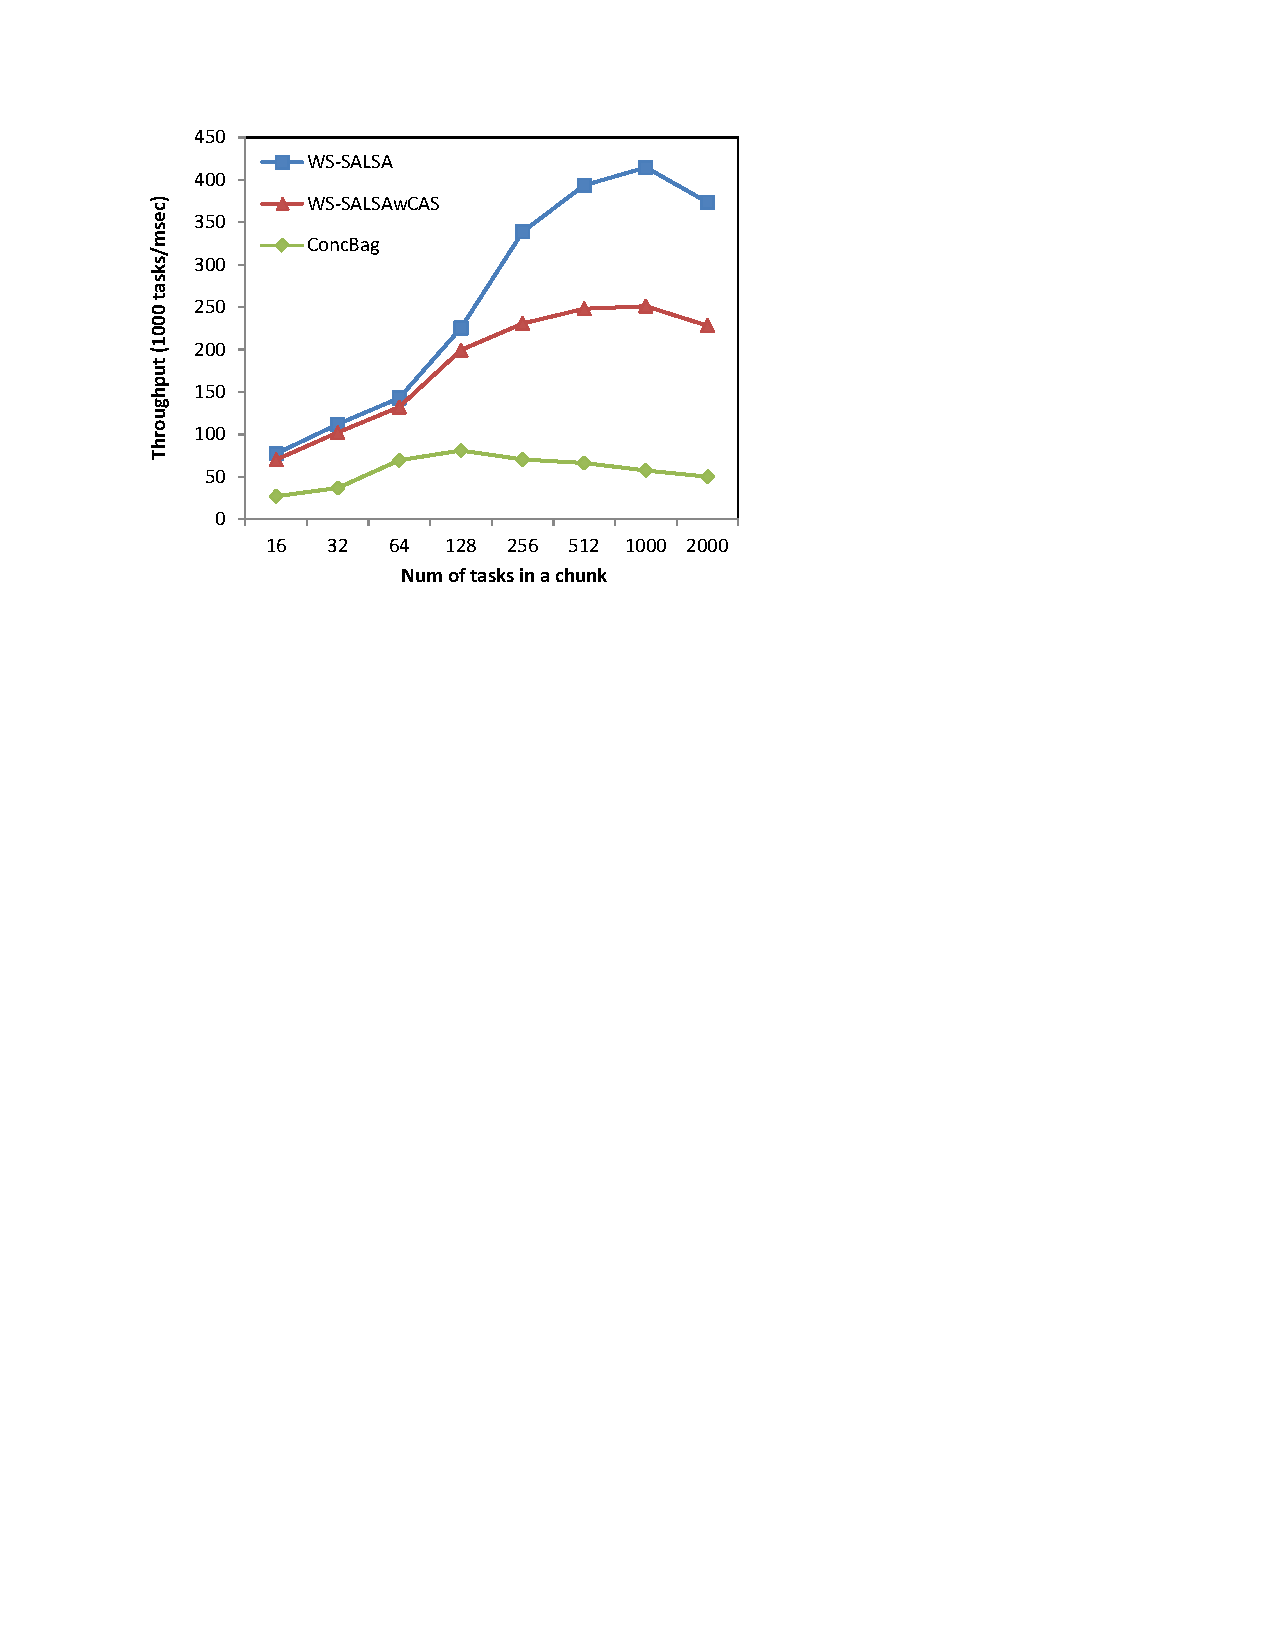
\includegraphics[width=0.5\textwidth]{figures/chunk-size}
 \end{center}
\caption{\footnotesize{System throughput as a function of chunk size. }}
	\label{fig:chunk-size}
\end{figure}
Figure~\ref{fig:chunk-size} shows the effect of chunk size on system throughput, for SALSA, SALSA+CAS and ConsBags, in the 16 producers / 16 consumers scenario. From this graph we can conclude that the optimal chunk size for SALSA and SALSA+CAS is 1000, while the optimal chunk size for ConsBags is 128. We believe that the reason that ConsBags cannot handle large task sizes is because when as consumer gets a new chunk it first has to find the first task in that chunk by scanning it, while SALSA hold a pointer to the next available task. In our evaluation we used to optimal chunk size for all the algorithms.
